%%%%%%%%%%%%%%%%%%%%%%%%%%%%%%%%%%%%%%%%%%%%%%%%%%%%%%%%%%%%

\section{Exploring \Wikipedia{} with \WikiTax} 
\label{S:tool}

\paragraph*{\textbf{\Wikipedia's category graph}}

\Wikipedia{} uses several means of organizing its information: plain links giving rise to an article graph, designated article lists, portals meant to introduce users to key topics, info-boxes for semantic (`typed') data, and categories giving rise to a category graph for the classification of articles. When it comes to taxonomy mining, the category graph is particularly relevant; the graph is accessible, for example, through the \MediaWiki{} API\footnote{\url{http://www.mediawiki.org/wiki/API:Main_page}}, which is the access path chosen by \WikiTax.

%%%%%%%%%%%%%%%%%%%%%%%%%%%%%%%%%%%%%%%%%%%%%%%%%%%%%%%%%%%%

\paragraph*{\textbf{Graph extraction and reduction with \WikiTax}}

Initially, \WikiTax{} is pointed to a root category (level 0) for
extraction. Iteratively, subcategories and pages (in fact, page
titles) can be extracted level by level or exhaustively. Exhaustive
extraction may take minutes to hours depending on the root
category. The \Wikipedia{} category graph contains many surprising
edges, which would easily imply inclusion of large, arguably
irrelevant subgraphs. Thus, extraction needs to be controlled.

\WikiTax{} supports reduction of the graph---both during
(level-by-level) extraction and post extraction. Reduction is based on
the selection of edges for exclusion. If all edges to a given category
are excluded, then the corresponding category node is also effectively
excluded. (We note that a category may have multiple parent
categories.) When reduction is performed during extraction, then the
excluded edges (nodes) are not followed by subsequent extraction
steps. When reduction is performed post extraction, then edges are
only blacklisted so that all decisions can be easily revised later.

%%%%%%%%%%%%%%%%%%%%%%%%%%%%%%%%%%%%%%%%%%%%%%%%%%%%%%%%%%%%

\begin{figure}[t!]
\begin{center}
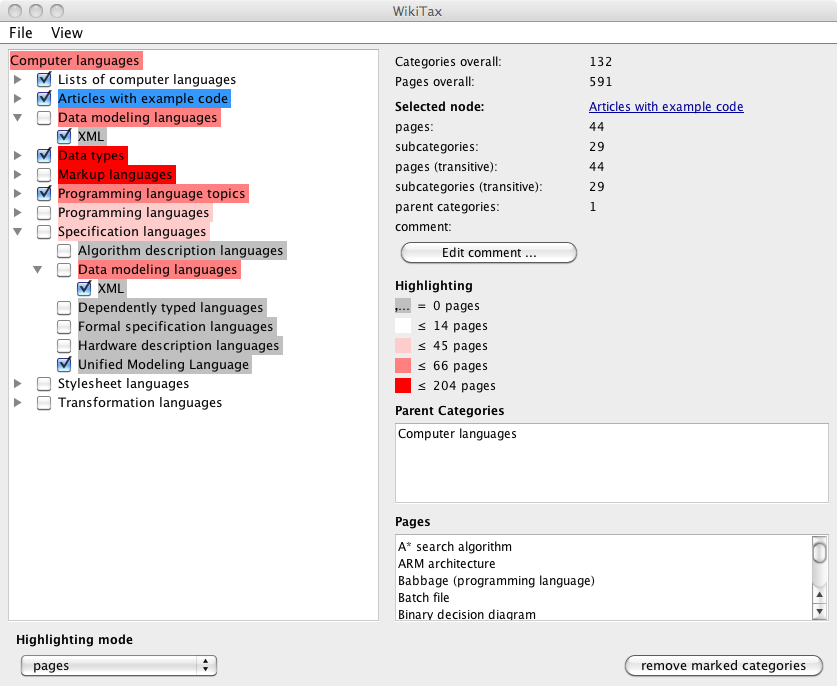
\includegraphics[width=.84\textwidth]{figures/clLevel12.png}
\end{center}
\vspace{-66\in}
\caption{Exploration of level 1 and 2 subcategories of \emph{Computer languages}.}
\label{F:clLevel12}
\vspace{-42\in}
\end{figure}

%%%%%%%%%%%%%%%%%%%%%%%%%%%%%%%%%%%%%%%%%%%%%%%%%%%%%%%%%%%%

\autoref{F:clLevel12} shows the \WikiTax{} exploration view after the
extraction of two levels (level 1 and 2) starting from the category
\WikipediaCategory{Computer languages}. Some edges are selected for
exclusion. (Exclusion happens upon pushing the
`removal/blacklist' button.)  In \S\ref{S:study}, we discuss reasons
for exclusion systematically, but it suffices here to say that the
selected categories are not proper language classifiers in a certain
narrow sense. Highlighting is applied to the categories according to
the metric of immediate member pages. We have selected the category
\WikipediaCategory{Articles with example code} for which some extra
data is shown in the panel on the right. All categories and pages are
clickable to navigate to \Wikipedia.

%%%%%%%%%%%%%%%%%%%%%%%%%%%%%%%%%%%%%%%%%%%%%%%%%%%%%%%%%%%%

\begin{figure}[ht]
\centering
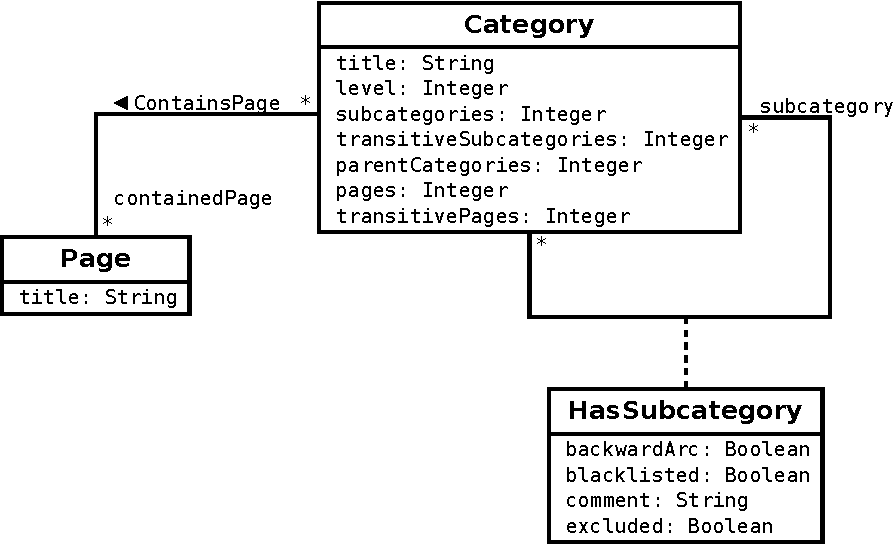
\includegraphics[width=0.63\textwidth]{../manual/figures/full_schema.pdf} 
\caption{Metamodel of the \WikiTax{} category graph.}
\label{F:metamodel}
\vspace{-42\in}
\end{figure}

%%%%%%%%%%%%%%%%%%%%%%%%%%%%%%%%%%%%%%%%%%%%%%%%%%%%%%%%%%%%

\WikiTax{} operates on an enhanced category graph; see the metamodel in \autoref{F:metamodel}. Thus, each category associates with contained pages and subcategories. The subcategory associations are attributed to keep track of metadata as follows: 

\vspace{-22\in}

{\small

\begin{description}
\item[backwardArc] Marker for cyclic edges in the category graph.
\item[blacklisted] Marker for categories blacklisted past extraction.
\item[excluded] Marker for categories excluded during reduction.
\item[comment] Label (`reason for exclusion') to be associated with the edge.
\end{description}

}

\vspace{-22\in}

\noindent
Categories are associated with measures as follows:

\vspace{-22\in}

{\small

\begin{description}
\item[level] The level 0, 1, 2, ... of the category in the graph with the root at level 0.
\item[subcategories] The number of immediate subcategories.
\item[transitiveSubcategories] The number of all subcategories.
\item[pages] The number of immediately contained pages.
\item[transitivePages] The number of all pages in this category.
\end{description}

}

\vspace{-22\in}

\noindent
Internally, \WikiTax{} uses the Java-based JGraLab
library\footnote{\url{https://github.com/jgralab}} for the
representation of (annotated) graphs with JSON as an export
format.

%%%%%%%%%%%%%%%%%%%%%%%%%%%%%%%%%%%%%%%%%%%%%%%%%%%%%%%%%%%%
